\section{向量}
    \subsection{概念}
    向量就是有方向的量,屬於高二數學。有兩種方式可以表達一個向量,
    用箭頭或一串數字。

    \begin{figure}[!htbp]
        \centering
        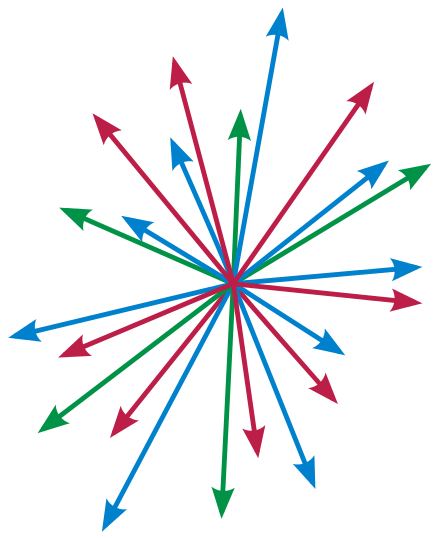
\includegraphics[width=0.2\textwidth]{../Images/Vector.png}
    \end{figure}

    $$
    \vec{v}=(x_1,x_2, \cdots ,x_n)
    $$

    在線性代數當中,我們將向量抽象化,不過我們暫時不會注意這一點,
    因為會用到非歐空間的向量的題目通常都非常困難。

    在資訊競賽上,我們最常使用的是平面向量,而座標平面上的點可以視為
    從$(0,0)$開始到那一個點的向量。

    \subsection{基本運算}
    向量可以支援幾種運算,加,加法反元素,減,係數積,向量長度,內積。

    首先是加法,若不考慮圖形,向量的加法定義是所有座標分別相加。

    $$\vec{v}=(v_1,v_2, \cdots ,v_n) , \; \vec{u}=(u_1,u_2, \cdots ,u_n)$$

    $$v+u=(v_1+u_1,v_2+u_2, \cdots ,v_n+u_n)$$

    加法反元素$v^{-1}$定義為$v+v^{-1}=\vec{0}$,也就是$-v$。

    減法就是加上那一個向量的加法反元素。

    係數積表達了對向量的一個伸縮,如果$k \in \R$為係數。

    $$kv=(kv_1,kv_2, \cdots ,kv_n)$$

    向量長度就是向量到原點的距離。

    $$\vec{v}=(v_1,v_2, \cdots ,v_n), \; |v|=\sqrt{v_1^2,v_2^2, \cdots ,v_n^2}$$

    內積的定義是一個向量的長度,乘上另一個向量在他上面的投影長。

    $$v \cdot u = |v| \times |u| \times \cos \theta$$

    其中,$\theta$是兩個向量的夾角。

    可以證明 $v \cdot u = v_1 \times u_1+v_2 \times u_2+ \cdots +v_n \times u_n$

    \begin{proof}
        $$v=(v_1,v_2, \cdots ,v_n),u=(u_1,u_2, \cdots ,u_n)$$

        $$|v|=\sqrt{v_1^2,v_2^2, \cdots ,v_n^2},|u|=\sqrt{u_1^2,u_2^2, \cdots ,u_n^2}$$
        
        $$|v|^2=v_1^2,v_2^2, \cdots ,v_n^2,|u|^2=u_1^2,u_2^2, \cdots ,u_n^2$$
        
        \begin{align*}
            |v-u|^2 &=(v_1-u_1)^2,(v_2-u_2)^2, \cdots ,(v_n-u_n)^2 \\
            &=\sum_{i=1}^{n} (v_i-u_i)^2 \\ 
            &=\sum_{i=1}^{n} (v_i^2+u_i^2-2\times v_i \times u_i) 
        \end{align*}

        \begin{align*}
            \cos \theta &= \frac{|v|^2+|u|^2-|v-u|^2}
            {2\times |v| \times |u|} \\
            &=\frac{\sum\limits_{i=1}^{n} v_i^2+ \sum\limits_{i=1}^{n} u_i^2- \sum\limits_{i=1}^{n} (v_i^2+u_i^2-2\times v_i \times u_i)}
            {2\times |v| \times |u|} \\
            &=\frac{\sum\limits_{i=1}^{n} (2\times v_i \times u_i)}
            {2\times |v| \times |u|} \\
            &=  \frac{\sum\limits_{i=1}^{n} (v_i u_i)}{|v||u|} \\
        \end{align*}

        \begin{align*}
            v \cdot u &= |v||u|\cos \theta = |v||u| \times \frac{\sum\limits_{i=1}^{n} (v_i u_i)}{|v||u|} \\
            &=\sum_{i=1}^{n} (v_i \times u_i)
        \end{align*}
    \end{proof}

    \subsection{實作}
    我們會使用一個struct方便我們使用2D Vector。

\begin{lstlisting}[caption=2D vector]
using T=long long;
struct Pt {// point
    T x,y;

    Pt()        { x=0, y=0;}
    Pt(T a,T b) { x=a, y=b;}

    void operator+=(const Pt a) { x+=a.x, y+=a.y;}
    void operator-=(const Pt a) { x-=a.x, y-=a.y;}
    void operator*=(const T a)  { x*=a, y*=a;}
    bool operator==(const Pt b) { return x==b.x && y==b.y;}
    bool operator!=(const Pt b) { return x!=b.x || x==b.y;}

    Pt operator+(const Pt a) { return Pt(x+a.x,y+a.y);}
    Pt operator-(const Pt a) { return Pt(x-a.x,y-a.y);}
    Pt operator*(const T a)  { return Pt(x*a,y*a);}
    Pt operator/(const T a)  { return Pt(x/a,y/a);}

    double len() {
        return sqrt(x*x + y*y);
    }

    T norm() {
        return x*x + y*y;
    }
};

T dot(const Pt a, const Pt b)  { return a.x*b.x + a.y*b.y;}
\end{lstlisting}

